\documentclass{standalone}
\usepackage{pgfplots}
\pgfplotsset{compat=1.16}
\begin{document}
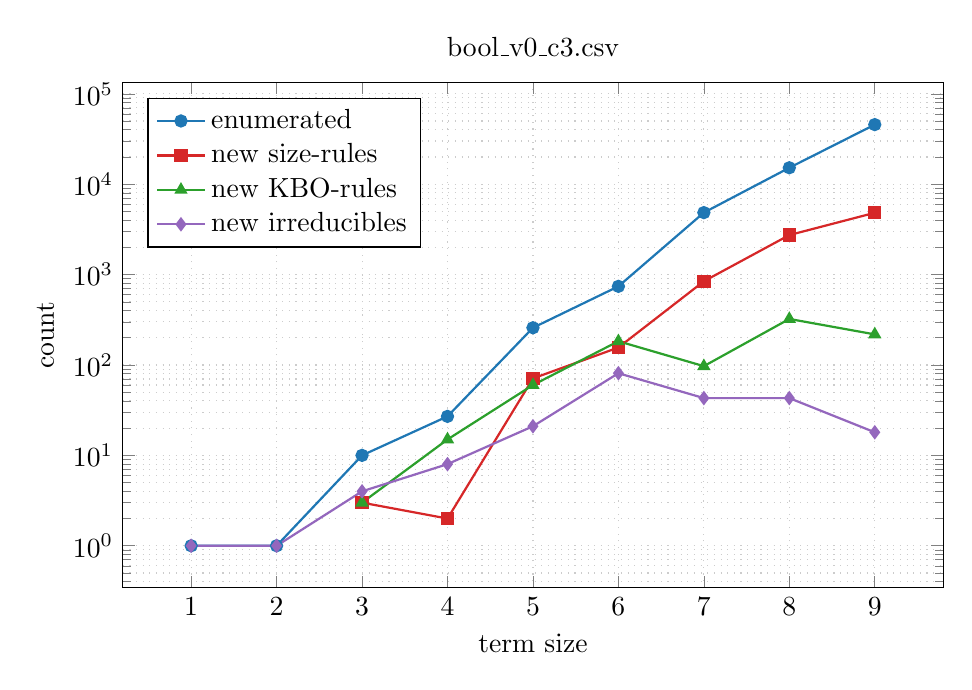
\begin{tikzpicture}
  \begin{axis}[
      width=12cm, height=8cm,
      xlabel={term size},
      ylabel={count},
      title={bool\_v0\_c3.csv},
      ymode=log,
      grid=both,
      grid style={dotted, gray!40},
      legend pos=north west,
      legend cell align=left,
      mark size=2pt,
    ]
    \definecolor{cenumerated}{HTML}{1f77b4}
    \addplot[color=cenumerated, mark=*, thick] coordinates {(1,1) (2,1) (3,10) (4,27) (5,258) (6,741) (7,4846) (8,15193) (9,45605)};
    \addlegendentry{enumerated}
    \definecolor{cnewsizerules}{HTML}{d62728}
    \addplot[color=cnewsizerules, mark=square*, thick] coordinates {(1,0) (2,0) (3,3) (4,2) (5,71) (6,156) (7,843) (8,2736) (9,4825)};
    \addlegendentry{new size-rules}
    \definecolor{cnewkborules}{HTML}{2ca02c}
    \addplot[color=cnewkborules, mark=triangle*, thick] coordinates {(1,0) (2,0) (3,3) (4,15) (5,60) (6,183) (7,97) (8,323) (9,218)};
    \addlegendentry{new KBO-rules}
    \definecolor{cnewirreducibles}{HTML}{9467bd}
    \addplot[color=cnewirreducibles, mark=diamond*, thick] coordinates {(1,1) (2,1) (3,4) (4,8) (5,21) (6,81) (7,43) (8,43) (9,18)};
    \addlegendentry{new irreducibles}
  \end{axis}
\end{tikzpicture}
\end{document}
